\documentclass[a4paper,11pt]{article}

\usepackage{setspace}
\onehalfspacing

\usepackage[utf8]{inputenc}
\usepackage[T1]{fontenc}
\usepackage[english]{babel}

\usepackage{color}
\usepackage{float}
\usepackage{fancyvrb}

\usepackage{amssymb}
\usepackage{amsmath}
\usepackage{listings}
\usepackage{comment} 

\usepackage{caption}
\usepackage{subcaption}

\usepackage{graphicx}
\DeclareGraphicsExtensions{.jpg}

\definecolor{dkgreen}{rgb}{0,0.45,0}
\definecolor{gray}{rgb}{0.5,0.5,0.5}
\definecolor{mauve}{rgb}{0.30,0,0.30}

\lstset{frame=tb,
  language=Python,
  aboveskip=3mm,
  belowskip=3mm,
  showstringspaces=false,
  columns=flexible,
  basicstyle={\small\ttfamily},
  numbers=left,
  numberstyle=\footnotesize,
  keywordstyle=\color{dkgreen}\bfseries,
  commentstyle=\color{dkgreen},
  stringstyle=\color{mauve},
  frame=single,
  breaklines=true,
  breakatwhitespace=false,
  tabsize=1
}

\begin{comment}
\begin{lstlisting}[language=python]
her kan i vise kode som i forklarer.
indryk virker fint her.
\end{lstlisting}
\end{comment}

\title{First year project\\Project 99: Who's Julia?\\\rule{10cm}{0.5mm}}
\author{Group: 99a\\Simon Lehmann Knudsen, simkn15\\Sonni Hedelund Jensen, sonje15\\Asbjørn Mansa Jensen, asjen15
	\\ DM501\\\rule{5.5cm}{0.5mm}\\}
\date{\today}

\begin{document}

\maketitle

\vfill

\newpage
\tableofcontents

\newpage
\section{Introduction}
Julia is a new open source object orientated programming language which shares many similarities with python. The language is made for high performance and scientific computations while still supporting general purpose programming. 

\subsection{Syntax}
\textit{Make examples of syntax between all the languages here}.

\subsection{Features}
Julia supports the following: Multiple dispatch and dynamic typing. The dynamic type system is similar to python. A property of dynamic typing is the type checks which are performed at runtime, mostly - opposed to static typing which makes the type checks at compile time. In Julia it is possible to specify types but for the most part it is not necessary because of the dynamic type system. Julia makes decisions about what size to assign to the variables which does not change at run time and cannot be changed after initialization. The types that are supported in Julia:
\begin{description}
	\item[$\cdot$] Signed / unsigned integers of; 8, 16, 32, 64 and 128 bits.
	\item[$\cdot$] Floating points of 16, 32 and 64 bits.  
	\item[$\cdot$] Boolean – 8 bits 
	\item[$\cdot$] Char – 32 bits 
\end{description}

Julia will by default assign 32 bits to an integer or floating if no more memory is needed at initialization. Julia has abstract types – an abstract type is just some from of generalization of a certain type. For example 16, 32 and 64 bit floats are an AbstractFloat. This is especially useful when the programmer doesn't know how much memory a certain variable may need. Too little memory will result in a bug and too much memory is a waste. Multiple dispatch is used to determine which function to call by the type of one or more of the parsed argument(s). This is useful when, e.g. two functions with the same name are declared:

\begin{lstlisting}[language=python]
function a(arg1::Int8)
	println("Int")  
end

function a(arg1::Float16)  
	println("Float")  
end    
\end{lstlisting}

If a variable is declared with a type of Int8 and parsed to the function a(...), then it will print "Int", and if the variable is declared as Float16 it will print "Float". It is also possible to use abstract types here, so arg1::Float16 and arg1::Int8 could be changed to arg1::AbstractFloat and arg1::AbstractInt – this will make the function 'a' accept any kinds of floats and ints.  
User defined types: User defined types, also known as composite types which gives the option to define new types. A composite type in Julia may look something like the following: 
\begin{lstlisting}[language=python]
type person 
	age::Int16 
	name 
end    
\end{lstlisting}
If a variable in a composite type is not specified with any type, the default is ::Any which accepts any kinds of types. To initialize a composite type you can treat it like an object. Person = person(21, "Carl"), and the values can be changed with "Person.age = 25". The developers of Julia states that user defined types are as fast and compact as built in types. 

\subsubsection{Garbage Collector}
Julia uses a garbage collector to automatically free the memory when needed. There is no guarantee when the garbage collector will run, but is it possible to force garbage collection with a function call: \textbf{gc()}. One thing to keep in mind is that once a name is defined in Julia, it will always be present till termination. The garbage collector doesn't free the memory of unreachable object but rather reallocates memory for objects when memory size has changed. So the only way the garbage collector can free memory is when an object has been reduced in size, for example:

\begin{lstlisting}[language=python]
A = rand(float32, 10000, 10000) 
A = 0
Gc() 
\end{lstlisting}
This code will generate a 10000x10000 matrix filled with random 32 bit floating points which consumes a bit of memory. \textbf{A} will be set to 0 but will keep the memory size of the 10000x10000 matrix until garbage collection is done either manually as in this example or somewhere in the future when it is done automatically. 

\subsubsection{Built-in package manager}
Julia comes with a built in package manager which keeps track of which packages that needs to be included in the users program to run, so is it not necessary to state which packages that need to be included. For example when the user calls the sort function, \textbf{sort()}, no package include statement or \textbf{math.sort()} is needed – this is done automatically by the package manager.

\subsubsection{Lightweight green threading}
A thread is lightweight when it shares address space with other threads opposed to heavyweight threads which has its own address space. If threads share the same address space the communication between them is faster and much simpler. The communication between heavyweight threads have to go through pipes or sockets. Green threads are threads that are scheduled not by the operating system but rather by the runtime library or virtual machine. Green threads does not have to relay on the operating system and can be controlled much better – the threads are in user space and not kernel space. As of Julia 0.4.5 multithreading is not available but in the unstable version 0.5.0 an experimental support of multithreading is available. 

\subsubsection{Meta-programming and Macros}
Meta-programming is a way to write programs in programs and let them use program code as data. In Julia meta-programming can be done by defining macros. For example, the @time macro was used extensively in the project. The @time is in the standard Julia library. The @time takes a function as an argument and sets a timer in the top of the code from the argument and stops the timer in the bottom and prints the time passed and memory allocated. Meta-programming and macros are known from Lisp, a programming language, and have been used in early AI research. 

\subsubsection{Implementing code from other languages}
Since Julia is a newer language there are not many written libraries yet. Julia has an import feature for both Python and C libraries to avoid this disadvantage. Import the library PyCall with the "using" operation to use python and import Python libraries via a macro @pyimport. To use C libraries or coding, simply run the function ccall(). The programming language C is a well known and used language. Many systems are based on C, which makes C an advantage for hardware programming. Another feature is to execute shell commands. Execute shell commands using run(``). An example would be running run(`echo Hello World`) which would return the output "Hello World".

\section{Projecteuler 11}

\textit{In the 20x20 grid below, four numbers along a diagonal line have been marked in red. The product of these numbers is 26 x 63 x 78 x 14 = 1788696. What is the greatest product of four adjacent numbers in the same direction (up, down, left, right, or diagonally) in the 20x20 grid?}
\begin{figure}[H]
	\begin{center}
	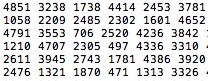
\includegraphics[scale=0.80]{11.jpg}
	\label{11}
	\end{center}
\end{figure}

The program runs from command-line/terminal in order to be able to test on different inputs and amount of adjacent numbers multiplied. To run the Julia version from the terminal: \textbf{Julia euler11.jl 100 4}. This would make the program run a matrix of size 100 and calculating product of 4 adjacent numbers. There was made a matrix generator, found in appendix, which makes a file with data to test. The file would be named \textbf{mat100.txt} for data to a $100 \cdot 100$ matrix. The numbers in the file ranging from 100-9999, 3-4 digit numbers. The original problem states two digit numbers in the data, but this would make a lot of duplicated numbers when testing with larger inputs, e.g. a $5000 \cdot 5000$ matrix. Some programming languages optimizes code during run time if it can predict what a given result will be. Having many duplicated numbers in the dataset could have an influence of the benchmarking between languages. To avoid this situation, to some extent, the digits have been increased. The algorithm first reads through a file with the input and makes a matrix. To calculate products in all directions needed in the problem, the algorithm goes through the matrix a total of 3 times. A nested for loop is needed to go though a matrix, lines 1-2 at figure \ref{111}. The outer loop iterates through the rows, and the inner loop iterates through the columns. Figure \ref{111} calculates the horizontal and vertical directions, firgure \ref{112} diagonally from left to right(downwards) and figure \ref{113} going diagonally from right to left(downwards). The algorithm starts in the most upper left cell, and iterates through all cells in the matrix. Lets have the first cell as (1,1), first number is row(\textbf{i}) and second number is column(\textbf{j}). Looking at figure \ref{111}, \textbf{matLength} is the size of the matrix, size = 100 would mean a matrix of size $100 \cdot 100$. \textbf{numProd} is the number of adjacent numbers multiplied together. For matrix with size 100, and multiplying four adjacent numbers, the algorithm would do the following in figure \ref{111}: 
\begin{list}{}{}
	\item Starting at cell (1,1) to the end which is cell (100, 100 - 4).
	\item Line 5-7: Loops over the adjacent cells and multiplies the numbers.
	\item Line 8-10: Sets current product to max product, if current is larger than previously max product.
\end{list}
\begin{figure}[H]
	\begin{center}
		\lstinputlisting[linerange={22-38}]{euler11.jl}
		\caption{Horizontal and vertical}
		\label{111}
	\end{center}
\end{figure}
Figure \ref{112} shows the loop that iterates over the matrix and calculating the product of the diagonal going downwards from left to right. Figure \ref{113} shows the diagonal product going upwards from left to right. The loop starts in the first row, and starting column is the last, not the first like the previously loops.
\begin{figure}[H]
	\begin{center}
		\lstinputlisting[linerange={43-51}]{euler11.jl}
		\caption{Diagonal downwards left to right}
		\label{112}
	\end{center}
\end{figure}
\begin{figure}[H]
	\begin{center}
		\lstinputlisting[linerange={56-64}]{euler11.jl}
		\caption{Diagonal upwards left to right}
		\label{113}
	\end{center}
\end{figure}

\section{Projecteuler 116}
Description: A row of five black square tiles is to have a number of its tiles replaced with coloured oblong tiles from red(length two), green(length three), or blue(length four). If red tiles are chosen there are exactly seven ways. If green tiles are chosen there are three ways. And if blue tiles are chosen there are two ways. Figure \ref{116} is a visualization of how the tiles can be lain. Assuming that colours cannot be mixed there are $7+3+2=12$ ways of replacing the black tiles in a row measuring five units in length. How many different ways can the black tiles in a row measuring fifty units in length be replaced if colours cannot be mixed and at least one coloured tile must be used?

\begin{figure}
	\centering
	\begin{subfigure}[b]{0.6\textwidth}
		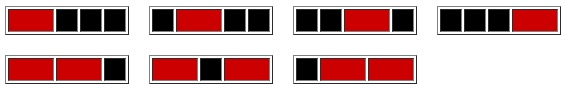
\includegraphics
		[width=\textwidth]{1161.jpg}
		\caption{Red tiles}.
	\end{subfigure}
	\begin{subfigure}[b]{0.6\textwidth}
		\centering
		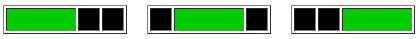
\includegraphics
		[width=\textwidth]{1162.jpg} 
		\caption{Green tiles}.
	\end{subfigure}	
	\begin{subfigure}[b]{0.6\textwidth}
		\centering
		
\includegraphics
		[width=\textwidth]{1163.jpg} 
		\caption{Blue tiles}.
	\end{subfigure}
	\caption{Projecteuler: 116}
	\label{116}
\end{figure}


\section{Quicksort}
Quicksort applies the divide-and-conquer paradigm to sort numbers. Divide-and-conquer has three steps. \textbf{Divide} the problem into a number of subproblems that are smaller instances of the same problem. \textbf{Conquer} the subproblems by solving them recursively. If the subproblems sizes are small enough, however, just solve the subproblems in a straightforward manner. \textbf{Combine} the solutions to the subproblems into the solution for the original problem \cite[chapter 4, page 65]{cormen}. Description of quicksort: \cite[chapter 7, page 170-171]{cormen}
\begin{list}{}{}
	\item \textbf{Divide}: Partition (rearrange) the array A[p..r] into two (possible empty) subarrays A[p..q-1] and A[q+1..r] such that each element of A[p--q1] is less than or equal to A[q], which is, in turn, less than or equal to each element of A[q+1..r]. Compute the index q as part of this partitioning procedure.
	\item \textbf{Conquer}: Sort the two subarrays A[p..q-1] and A[q+1..r] by recursive calls to quicksort.
	\item \textbf{Combine}: Because the subarrays are already sorted, no work is needed to combine them: the entire array A[p..r] is now sorted.
\end{list}
Figure \ref{qs} shows a visualization of quicksort.
\begin{figure}
	\begin{center}	
		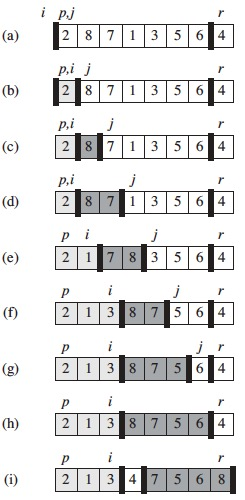
\includegraphics[scale=0.5]{qs.jpg}
		\caption{Quicksort}
		\label{qs}
	\end{center}
\end{figure}

\section{Statistics}

\section{Learning / Personal experience}
Some of the design choices, in Julia, can be really frustrating. The indexes starts at 1 - this could be debatable because of the statement that Julia is used in a lot of scientific computations. As a programmer who is used to indexes starting at 0, this can cause a lot of bugs. The developers of Julia made a weird design choice to the for-loop. A incrementing for loop looks like:
\begin{lstlisting}[language=python]
Julia:
for i = 1 : n
	Some code ...
end

General languages:
for i = 1; i < n; i++
	Some code ...
\end{lstlisting}
This is straightforward like many other languages, but take a look at the decrementing for-loop:
\begin{lstlisting}[language=python]
Julia:
for i = n : -1 : 0
	Some code ...
end

General languages:
for i = n; i > 0; i--
	Some code
\end{lstlisting}
In Julia it is needed to swap the decrement declaration in to the middle of the arguments which is needed both versions, incrementing and decrementing. The decrementing for-loops both start at n, and stops at 0. This kind of syntax can be the cause of many bugs, and is not that easy to get eyes on.
The documentation of Julia is far from being great, which is a huge bump on the road to learning Julia. It feels far from complete. The documentation doesn’t explain much but instead gives some examples. Essential information are often lacking, e.g. what types is needed to parse for a given function. It might describe arguments are needed, but lacking to describe the arguments. An example from the documentation is the function \textbf{rand()} which is used to generate random numbers:

\begin{lstlisting}
rand( [ rng ] [ ,S ] [ , dims... ] )

	Pick a random element or array of random elements from the set of values specified by S; S can be:
	- an indexable collection (for example 1:n or ['x','y','z']), or  
	- a type: the set of values to pick from is then equivalent to typemin(S):typemax(S) for integers (this is not applicable to BigInt), and to [0,1) for floating point numbers;  
	S defaults to Float64.
\end{lstlisting} 
The argument \textbf{S} is explained, but does not mention anything about \textbf{rng} or \textbf{dims}.
Simple things like how to access data within an array at a specific index. This should be one of the first things in the Array section, but is described after about two pages of text. If you have experience in other programming languages, you might know what is needed to type a[index] but this isn’t so obvious for new programmers. It is clear that something has to be done to the documentation.  
A downside to Julia is its consistency. The developers has tried to remove some of the burden from the programmer with dynamic typing, package manager system etc., but with memory allocation and garbage collector it does not make much sense. The garbage collector does not free memory from unreachable object. Sizes of variables cannot be changed after declaration, and is not automatically increased if needed.

\section{Conclusion}
It can be difficult to make any conclusions by the benchmarking but it may give an idea of how Julia performs, compared to Java, Python and C++. One thing to keep in mind is that as of writing this report, Julia is in version 0.4.5 - it has yet to reach version 1.0.0 while the other languages are much older than Julia. This could mean that Julia might get even faster in the future.   

\newpage

\section{Appendix (source code)}

%\textbf{Sierpinski triangle program}
%\lstinputlisting[language=python]{sierpinski.py}
%\textbf{Binary tree program}
%\lstinputlisting[language=python]{binary.py}

\begin{thebibliography}{9}
	
	\bibitem{cormen}
	Thomas H. Cormen, Charles E. Leiserson, Ronald Rivest, Clifford Stein
	\emph{Introduction to Algorithms},
	Cambridge, Massachusetts,
	third edition,
	2009.
	
\end{thebibliography}

\end{document}

